\chapter{Description}

The pixel testboard unit \enquote{Pixel DTB} is a data acquisition board specifically designed for the CMS pixel detector \gls{ROC}.

\begin{figure}[hbtp]
    \begin{center}
	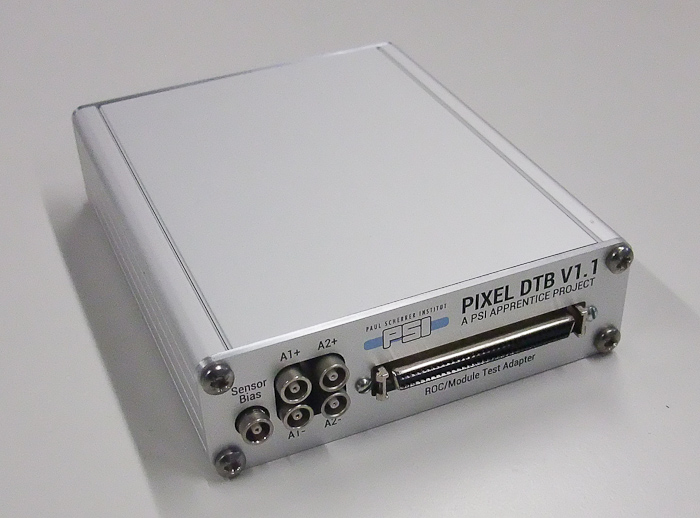
\includegraphics[width=0.7\textwidth]{img/DTB_front.jpg}

	\bigskip

	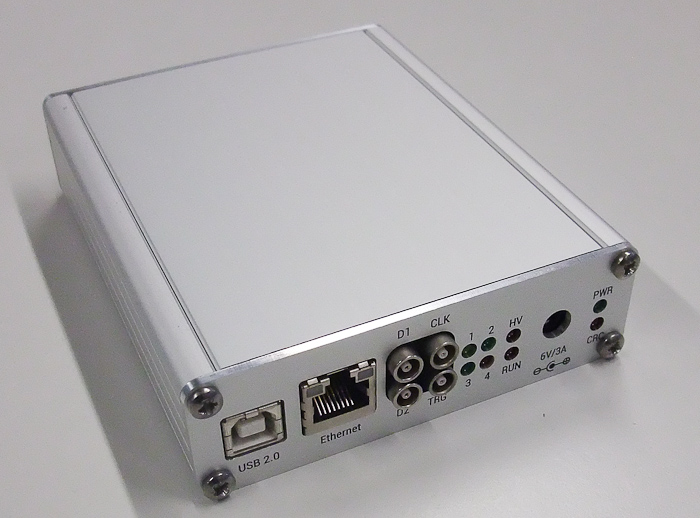
\includegraphics[width=0.7\textwidth]{img/DTB_back.jpg}
	\label{fig:DTBphoto}
	\caption{Photograph of the unit. Shown are the views from the front (top) and the rear (bottom). See text for a description of connectors.}
    \end{center}
\end{figure}

\begin{table}[p]
    \caption{Connector}
    {\tiny
	\begin{longtable}{cclll}
	    \toprule
	    \multicolumn{1}{l}{Conn} & \multicolumn{1}{l}{Cable} & Signal Name & Type & Description \\ 
	    \midrule
	    1 & 1 & GND & power & ground \\ 
	    35 & 2 & TIN\_p & LCDS out & token in (pos) \\ 
	    2 & 3 & TIN\_n & LCDS out & token in (neg) \\ 
	    36 & 4 & GND & power & ground \\ 
	    3 & 5 & nRESET & out & ROC reset not \\ 
	    37 & 6 & GND & power & ground \\ 
	    4 & 7 & SDATA1\_p & LCDS in & serial data channel 1 (pos); 400Mb/s, 160Mb/s, analog \\ 
	    38 & 8 & SDATA1\_n & LCDS in & serial data channel 1 (neg); 400Mb/s, 160Mb/s, analog \\ 
	    5 & 9 & GND & power & ground \\ 
	    39 & 10 & SDATA2\_p & LCDS in & serial data channel 2 (pos); 400Mb/s, analog \\ 
	    6 & 11 & SDATA2\_n & LCDS in & serial data channel 2 (neg); 400Mb/s, analog \\ 
	    40 & 12 & GND & power & ground \\ 
	    7 & 13 & SDATA3\_p & LCDS in & serial data channel 3 (pos); 400Mb/s \\ 
	    41 & 14 & SDATA3\_n & LCDS in & serial data channel 3 (neg); 400Mb/s \\ 
	    8 & 15 & GND & power & ground \\ 
	    42 & 16 & SDATA4\_p & LCDS in & serial data channel 4 (pos); 400Mb/s \\ 
	    9 & 17 & SDATA4\_n & LCDS in & serial data channel 4 (neg); 400Mb/s \\ 
	    43 & 18 & GND & power & ground \\ 
	    10 & 19 & CTR\_p & LCDS/LVDS out & combined calibrate trigger reset signal (pos) \\ 
	    44 & 20 & CTR\_n & LCDS/LVDS out & combined calibrate trigger reset signal (neg) \\ 
	    11 & 21 & GND & power & ground \\ 
	    45 & 22 & CLK\_p & LCDS/LVDS out & 40 MHz clock (pos) \\ 
	    12 & 23 & CLK\_n & LCDS/LVDS out & 40 MHz clock (neg) \\ 
	    46 & 24 & GND & power & ground \\ 
	    13 & 25 & VA+ & power & ROC/Module analog voltage \\ 
	    47 & 26 & VA+ & power & ROC/Module analog voltage \\ 
	    14 & 27 & VA+ & power & ROC/Module analog voltage \\ 
	    48 & 28 & VA+ & power & ROC/Module analog voltage \\ 
	    15 & 29 & VD+ & power & ROC/Module digital voltage \\ 
	    49 & 30 & GND & power & ground \\ 
	    16 & 31 & ROC\_A3 & out & ROC address bit 3 \\ 
	    50 & 32 & ROC\_A2 & out & ROC address bit 2 \\ 
	    17 & 33 & ROC\_A1 & out & ROC address bit 1 \\ 
	    51 & 34 & ROC\_A0 & out & ROC address bit 0 \\ 
	    18 & 35 & GND & power & ground \\ 
	    52 & 36 & SDA\_p & LCDS/LVDS out & ROC/Module I2C data (pos) \\ 
	    19 & 37 & SDA\_n & LCDS/LVDS out & ROC/Module I2C data (neg) \\ 
	    53 & 38 & GND & power & ground \\ 
	    20 & 39 & TOUT\_p & LCDS/LVDS in & ROC token out (pos) \\ 
	    54 & 40 & TOUT\_n & LCDS/LVDS in & ROC token out (neg) \\ 
	    21 & 41 & GND & power & ground \\ 
	    55 & 42 & VD+ & power & ROC/Module digital voltage \\ 
	    22 & 43 & VD+ & power & ROC/Module digital voltage \\ 
	    56 & 44 & VD+ & power & ROC/Module digital voltage \\ 
	    23 & 45 & VD+ & power & ROC/Module digital voltage \\ 
	    57 & 46 & GND & power & ground \\ 
	    24 & 47 & V33 & power & +3.3V \\ 
	    58 & 48 & V50+ & power & +5.0V \\ 
	    25 & 49 & V50- & power & -5.0V \\ 
	    59 & 50 & POWER\_ON & out & ROC/Module power status signal (H=power on; L=power off) \\ 
	    26 & 51 & I2C\_SCL2 & bidir & standard I2C master SCL to control periphery \\ 
	    60 & 52 & I2C\_SDA2 & bidir & standard I2C master SDA to control periphery \\ 
	    27 & 53 & IO0 &  & general purpose digital in/out 0 \\ 
	    61 & 54 & IO1 &  & general purpose digital in/out 1 \\ 
	    28 & 55 & IO2 &  & general purpose digital in/out 2 \\ 
	    62 & 56 & IO3 &  & general purpose digital in/out 3 \\ 
	    29 & 57 & AIN0 & analog in & general purpose analog input 0 to ADC \\ 
	    63 & 58 & AIN1 & analog in & general purpose analog input 1 to ADC \\ 
	    30 & 59 & AIN2 & analog in & general purpose analog input 2 to ADC \\ 
	    64 & 60 & GND & power & ground \\ 
	    31 & 61 & nc &  & HV spacer \\ 
	    65 & 62 & nc &  & HV spacer \\ 
	    32 & 63 & nc &  & HV spacer \\ 
	    66 & 64 & BIAS\_GND & power & sensor bias return \\ 
	    33 & 65 & nc &  & HV spacer \\ 
	    67 & 66 & nc &  & HV spacer \\ 
	    34 & 67 & nc &  & HV spacer \\ 
	    68 & 68 & BIAS & power & sensor bias \\ 
	    \bottomrule
	\end{longtable}
    }
    \label{ROCmoduleInterfaceConnector}
\end{table}


